\chapter{Query}

上一章主要讨论关系算子的实现问题，本章介绍SQL语句如何被翻译成算子表达式，算子表达式如何优化等问题。按照前一章所述，整个过程分为两步：生成逻辑执行计划，得到物理执行计划。详细的过程包括：
\begin{enumerate}
    \item 生成CST语法树
    \item CST上的预处理
    \item 生成算子表达式（或者抽象语法树AST）
    \item 优化逻辑执行计划
    \item 优化物理执行计划
\end{enumerate}

在SQL翻译阶段，主要利用编译原理的技术对SQL语句做词法、语法分析，得到一棵语法树，然后在语法树上做类型检查、视展开等预处理。这棵语法树需要被翻译成为算子表达式，算子表达式表现为AST抽象语法树。接下来需要变换算子表达式，目的是使算子表达式更容易计算，然后生成逻辑执行计划。最后选择算子实现算法，得到物理执行计划。逻辑执行计划与物理执行计划的优化方式有两种：一种是采用直观的规则，另一种是根据算法的性能做动态规划。

\begin{figure}[H]
    \centering
    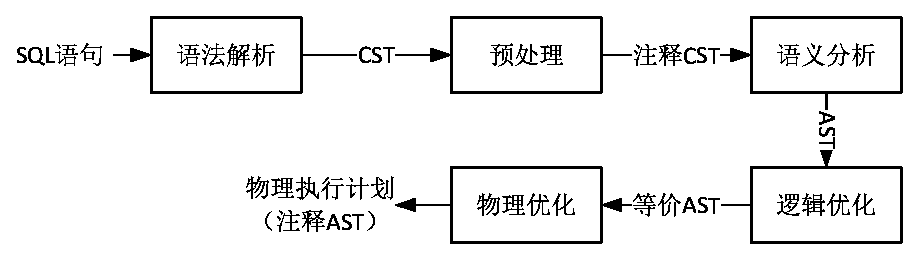
\includegraphics[width=\linewidth]{handout/img/6-process.eps}
    \caption{查询处理过程}\label{fig:6-process}
\end{figure}

\section{SQL语法解析}

在编译原理中，通常用正则表达式RE来描述词法，通过有限自动机FA来识别词法，有限自动机能识别的语言等价于正则表达式描述的语言。有限自动机输出为一个token流，在此基础上做语法解析。

当前绝大多数计算机语言使用上下文无关文法CFG来描述，使用堆栈下推自动机PDA来识别语法，二者也是等价的。CFG文法定义可能存在歧义，不能保证语法树的唯一性，并且理论上不存在判定CFG是否歧义的算法。另一方面，通用下推自动机PDA存在需要$O(n^3)$的复杂度来识别语法，这个复杂度太高了，人们追求的是在$O(n)$线性复杂度内识别语言。所幸的是，存在LL/LR这样的算法能够在线性复杂度识别某些CFG文法的结构，并且是保证无歧义。

\subsection{SQL子集文法}\label{sec:query-sql}

SQL语句按照语法规则被解析为一颗具体语法树CST。语法树的叶子节点称为\emph{终止符}，包括关键字、标识符、符号等，语法树的内部节点称为\emph{非终止符}。具体来说，终止符包括：1)~关键字，如\texttt{SELECT}、\texttt{WHERE}、\texttt{FROM}等；2)~对应于表名或者属性名的标识符；3)~表达式的各种符号，如\texttt{(}、\texttt{)}、\texttt{=}等。

这里以一个SQL子集文法作为示例，展示如何描述和识别SQL语言。这个子集没有包括\texttt{GROUP BY}、\texttt{ORDER BY}等产生式，完整的SQL语法定义可以参考\cite{SQLSynta19:online}。

这个SQL子集的语法产生式如下：

\begin{lstlisting}[style=verbose]
<Query> ::= SELECT <SelList> FROM <FromList> WHERE <Condition>
<SelList> ::= <Attribute>, <SelList>
<SelList> ::= <Attribute>
<FromList> ::= <Relation>, <FromList>
<FromList> ::= <Relation>
<Condition> ::= <Condition> AND <Condition>
<Condition> ::= <Attribute> IN ( <Query> )
<Condition> ::= <Attribute> = <Attribute>
<Condition> ::= <Attribute> LIKE <Pattern>
\end{lstlisting}

在SQL语法子集中，\texttt{<Query>}位于生成式左部，是一个非终止符，并且是整个语法生成式的根。\texttt{<Attribute>}、\texttt{<Relation>}、\texttt{<Pattern>}三个是终止符，词法分析器是无法判定这样的token类型的，必须在语义分析阶段由上下文来解释。\texttt{<Relation>}是指关系名称，\texttt{<Attribute>}指关系包含的属性名，\texttt{<Pattern>}指模式匹配的字符串。

按照语法规则，采用top-down或者bottom-up方法，将SQL语句解析为一颗具体语法树CST后，语法分析阶段就结束了，后面是语义分析阶段。

\begin{example}\label{exp:6-cst}
    假设有两张表定义如下：
\begin{lstlisting}[style=verbose]
    StarsIn(movieTitle, movieYear, starName)
    MovieStar(name, address, gender, birthdate)
\end{lstlisting}
在这两张表上执行查询语句：
\begin{lstlisting}[style=verbose]
    SELECT movieTitle
    FROM StarsIn
    WHERE starName IN (
        SELECT name
        FROM MovieStar
        WHERE birthdate LIKE '%1960'
    );
\end{lstlisting}
词法分析器首先扫描整个语句，识别token。\texttt{SELECT}被识别为一个关键字，token类型假设为1，然后movieTitle被识别成为一个关系属性，假设token类型为2。如此，当词法分析器识别一个token，然后输出token流。

语法分析器拿到token流后，根据LL或者LR语法解析程序，将token流装配成一棵具体语法树\figurename\ref{fig:6-cst}。注意这个查询语句是嵌套的，内层\texttt{SELECT}语句查询出一张表，然后使用\texttt{starName IN}表示相等。
\end{example}

\begin{figure}[H]
    \centering
    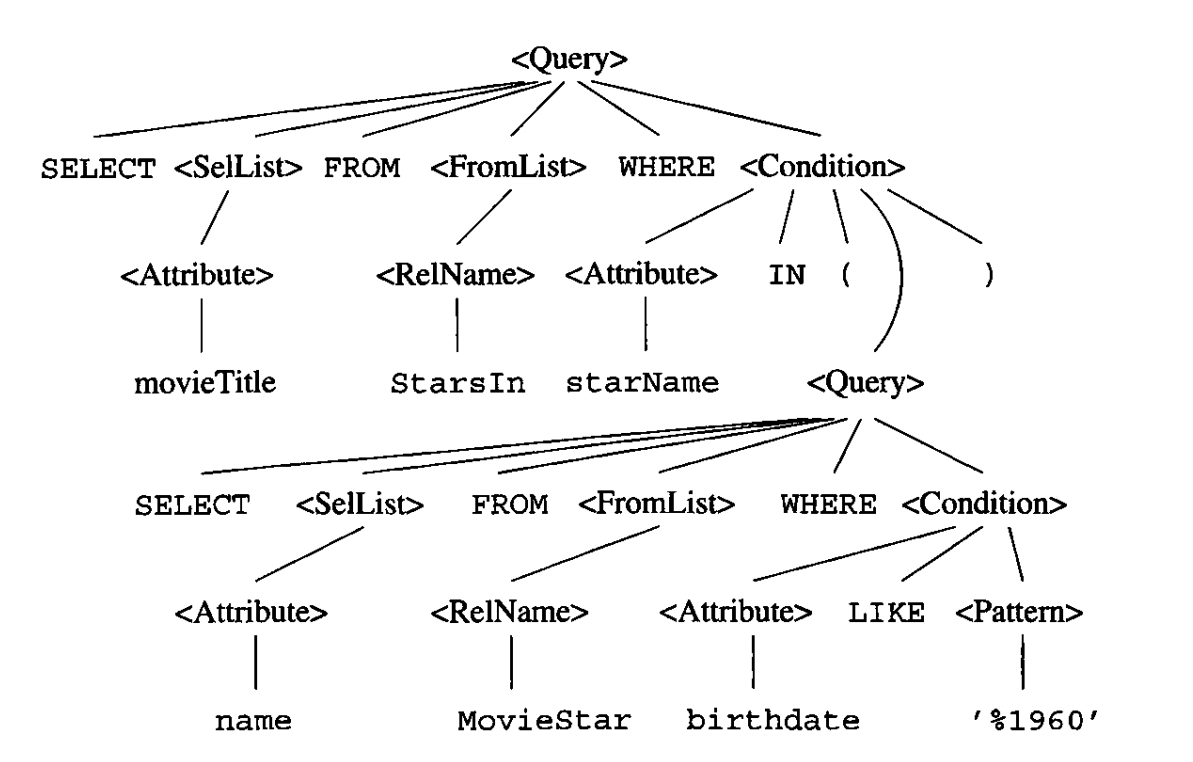
\includegraphics[width=\linewidth]{handout/img/6-cst.png}
    \caption{具体语法解析树CST}\label{fig:6-cst}
\end{figure}

\begin{example}\label{exp:6-cst2}
    \examplename\ref{exp:6-cst}采用嵌套方式查询，另一种方式采用多个条件的方式来查询：
\begin{lstlisting}[style=verbose]
    SELECT movieTitle
    FROM StarsIn, MovieStar
    WHERE starName = name AND birthdate LIKE '%1960';
\end{lstlisting}

    这个SQL语言被翻译成两个条件的组合，如\figurename\ref{fig:6-cst2}。
\end{example}

\begin{figure}[H]
    \centering
    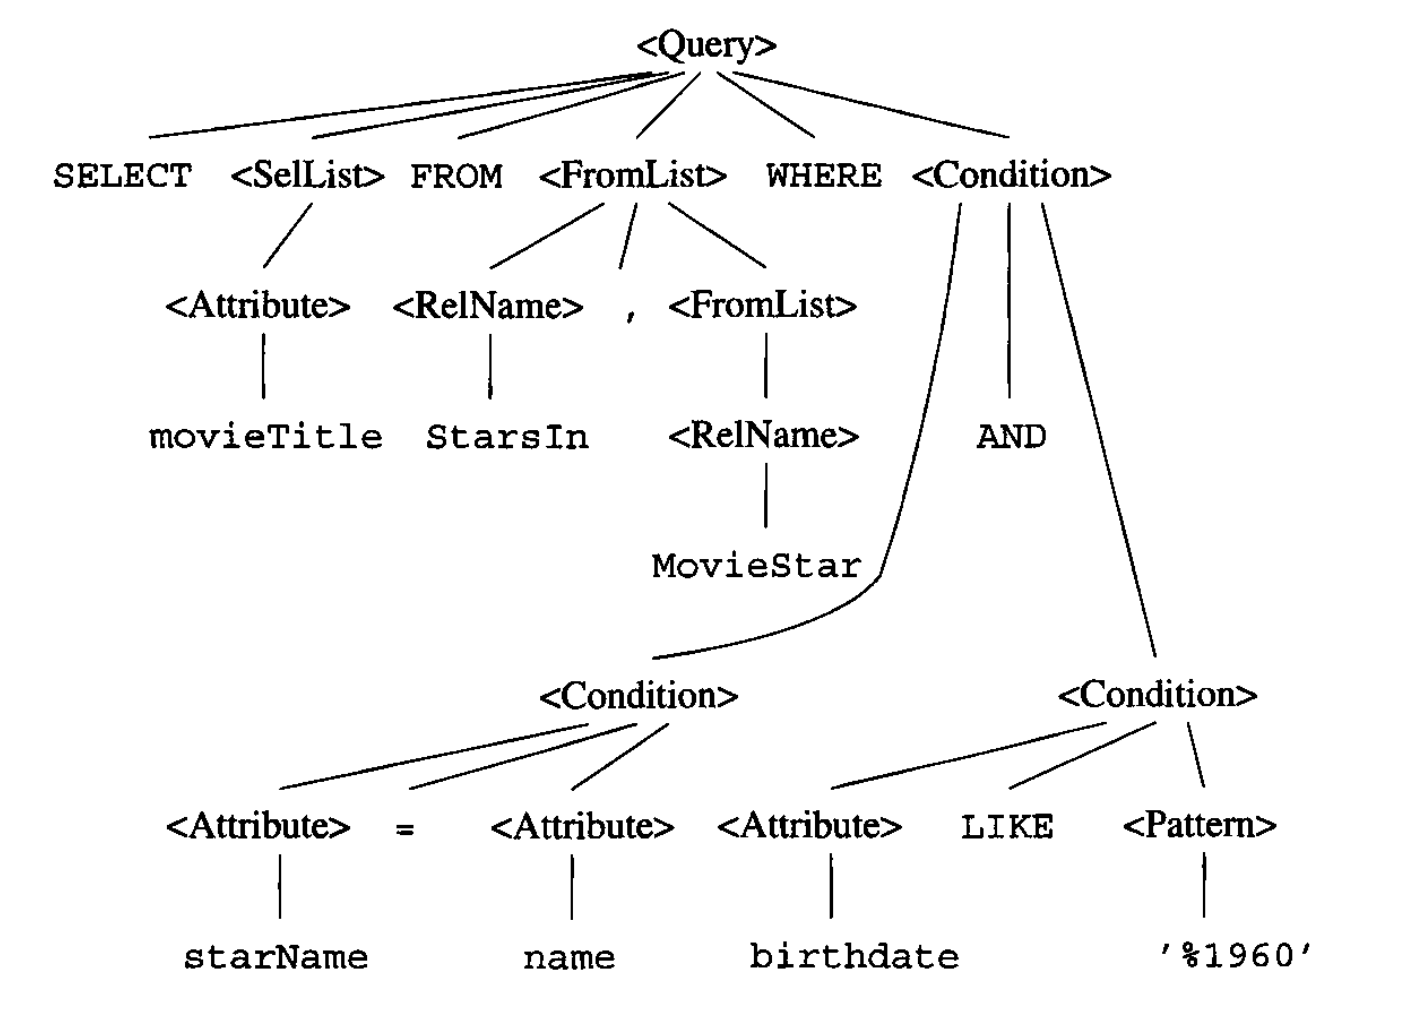
\includegraphics[width=\linewidth]{handout/img/6-cst2.png}
    \caption{具体语法解析树CST}\label{fig:6-cst2}
\end{figure}

\subsection{类型检查}

得到语法解析树CST后，接下来是语义分析，站在编译原理的角度，本章大部分的内容都是语义分析与优化。

一般来说，语义分析的第一步要检查变量的类型。与c语言不同，SQL语言没有变量声明，所以\examplename\ref{exp:6-cst}中\texttt{MovieStar}先被识别为某种类型的token，然后根据它在树中的位置确定为关系，去schema中查找是否有这样的关系。再去确定\texttt{name}是否出现在这个关系的属性中，检查条件判断中\texttt{birthdate}是否有这样的属性。

内部嵌套的这个\texttt{SELECT}语句输出为一个关系，这个关系的属性只有\text{name}字段。语句\texttt{WHERE starName IN}表示一个选择条件。

总结下来，类型检查的主要工作包括：
\begin{itemize}
    \item 检查from-list的关系变量是否有效
    \item 检查select-list或者condition的属性是否有效
    \item 检查类型，检查属性使用的类型是否满足各种计算的要求
\end{itemize}

类型检查围绕AST语法树做深度遍历，在树上做标记。一般的计算过程是先根据\texttt{<FromList>}生成式右部的\texttt{<Relation>}确定关系，然后再确定\texttt{<SelList>}和\texttt{<Condition>}中的属性，最后在\texttt{<Query>}节点上标注输出关系的属性集合。

\subsection{view展开}

在CST语法树上做类型检查时，还会碰到一些token为虚拟视view的情况。所谓视实际上是一条查询语句，SQL可以创建一个视，一个视并不一定意味着有底层存储的关系与之对应。如\figurename\ref{fig:6-view}，在语义解析时view需要展开成一段查询语句，效果上类似于嵌套查询。

\begin{figure}[H]
    \centering
    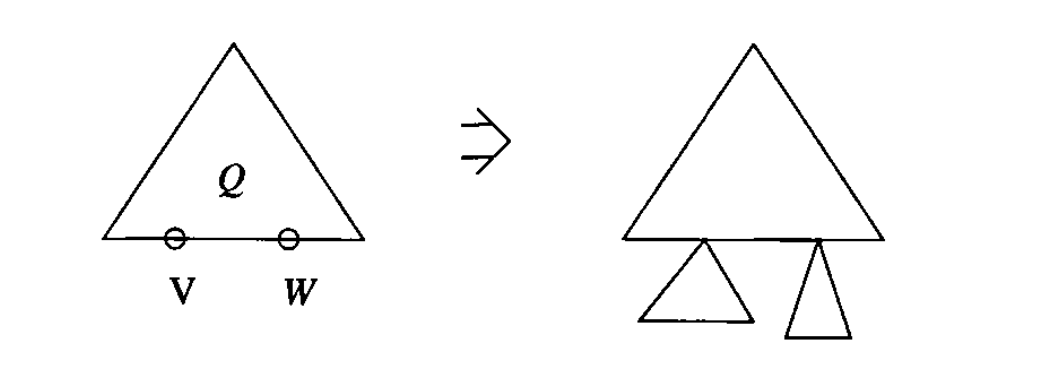
\includegraphics[width=0.5\linewidth]{handout/img/6-view.png}
    \caption{视的替换展开}\label{fig:6-view}
\end{figure}

view在某些数据库实现中会持久化为一张表，通过创建一些常用的视可以加快数据库查询过程，因为视可以看成是物化的中间结果。另外，教材中将类型检查与view展开都称为预处理是有道理的，它暗指这两个动作在一次CST遍历中处理。

\begin{example}\label{exp:6-view}
    利用下面的语句创建一个名为ParamountMovies的视：
\begin{lstlisting}[style=verbose]
    CREATE VIEW ParamountMovies AS
        SELECT title, year
        FROM Movies
        WHERE studioName = 'Paramount';
\end{lstlisting}

这个视的CST语法树表示为\figurename\ref{fig:6-view1}。假设有一条查询语句为：
\begin{lstlisting}[style=verbose]
    SELECT title
    FROM ParamountMovies
    WHERE year = 1979;
\end{lstlisting}

查询语句做语法解析后得到\figurename\ref{fig:6-view2}，对查询CST做深度遍历，如\figurename\ref{fig:6-view3}。遍历中，检查类型同时做view展开，最后得到\figurename\ref{fig:6-view4}。
\end{example}

\begin{figure}[H]
    \centering
    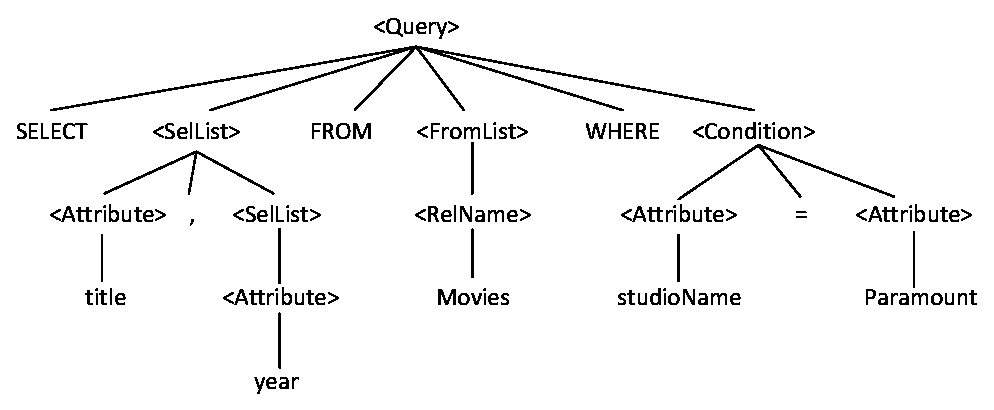
\includegraphics[width=\linewidth]{handout/img/6-view1.eps}
    \caption{view的CST}\label{fig:6-view1}
\end{figure}
\begin{figure}[H]
    \centering
    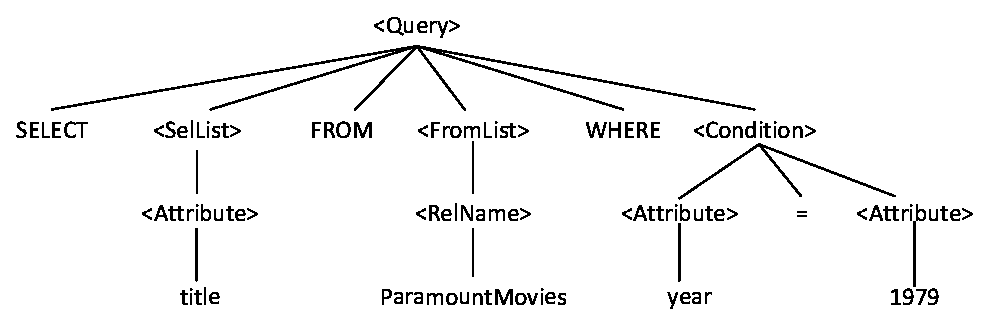
\includegraphics[width=\linewidth]{handout/img/6-view2.eps}
    \caption{查询CST}\label{fig:6-view2}
    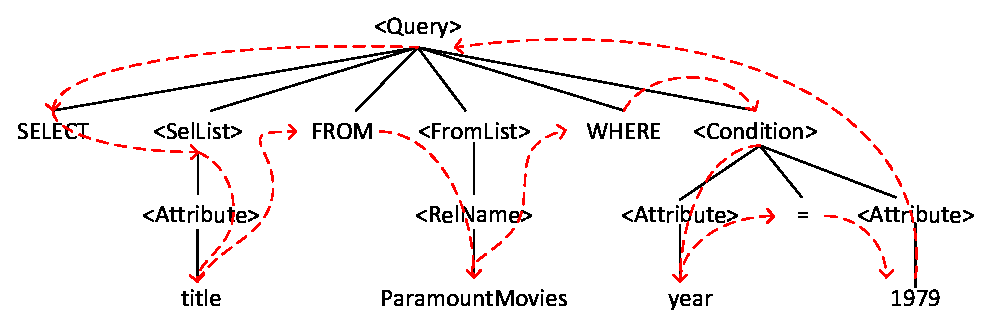
\includegraphics[width=\linewidth]{handout/img/6-view3.eps}
    \caption{深度遍历CST}\label{fig:6-view3}
    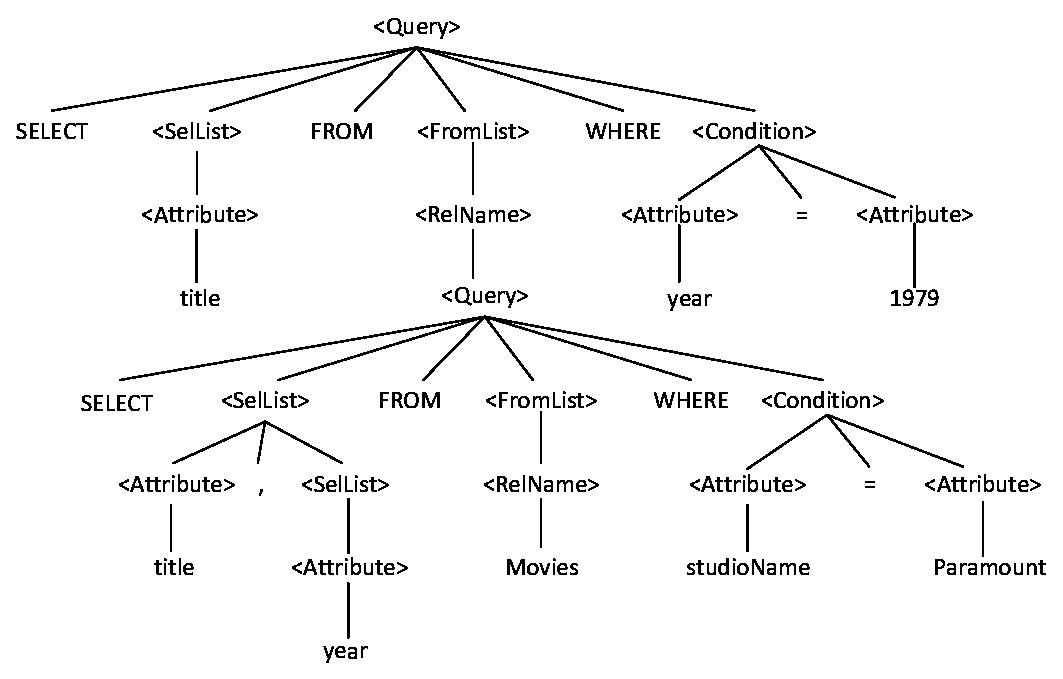
\includegraphics[width=\linewidth]{handout/img/6-view4.eps}
    \caption{视展开CST}\label{fig:6-view4}
\end{figure}

\section{算子表达式特性}

在CST语法树做完预处理后，下一步是要将查询语句翻译成算子表达式，这对应于一个抽象语法树AST。本节先讨论算子表达式的特性，下一节给出AST翻译方法。需要注意，所有关系运算的结果都是关系，换句话说关系代数是一个\emph{关系的封闭系统}。

\subsection{交换律与结合律}

只有双目算子能够考察交换性或结合性，单目算子不需要考虑。如果算子具有交换性与结合性，可将该算子的多次连续操作交换顺序，变换后的算子表达式仍然是等价的，这是一个常见的逻辑优化方案。

多数双目算子具有交换律和结合律，除了差$-$和$\theta$连接，并且适用于bag或者set模型：

\begin{itemize}
    \item $R \times S = S \times R$，$(R\times S) \times T = R\times (S\times T)$
    \item $R \bowtie S = S \bowtie R$，$(R \bowtie S) \bowtie T = R \bowtie (S \bowtie T)$
    \item $R \cup S = S \cup R$，$(R \cup S) \cup T = R \cup (S \cup T)$
    \item $R \cap S = S \cap R$，$(R \cap S) \cap T = R \cap (S \cap T)$
\end{itemize}

考虑等式左边的一个tuple一定会出现在等式的右边，容易证明以上规则。$\theta$连接$\bowtie_C$具有交换律，一般情况下没有结合律，除非$\bowtie_C$的条件在结合后有意义。
\begin{itemize}
    \item $R \bowtie_C S = S \bowtie_C R$
\end{itemize}

\begin{example}
    假设有三个关系$R(a,b)$、$S(b,c)$和$T(c,d)$，表达式$R \bowtie_{R.b>S.b} S \bowtie_{R.a<T.d} T$，条件$R.a<T.d$导致无法结合，因为$R.a$属性只出现在$R$和$R \bowtie_C S$中，$S$本身并没有这个属性。
\end{example}

如果为set模型，对并交操作满足分配律：
\begin{itemize}
    \item $A \cap_S (B \cup_S C) = (A \cap_S B) \cup_S (A \cap_S C)$
\end{itemize}
但是如果底层数据模型为bag，则$\cup_B$和$\cap_B$上不满足分配律。

\subsection{选择操作规则}

绝大多数数据库操作都是根据条件做tuple的查询，这对应于关系上的选择$\sigma$。$\sigma$算子能够穿透大多数双目算子，并且由于选择操作能够大幅降低中间计算结果尺寸，所以关系表达式最常见的逻辑优化规则是下推选择。

\vskip\baselineskip
第一组$\sigma$规则关于交、并、差三种双目算子，这三种算子要求操作关系的属性完全相同：
\begin{itemize}
    \item $\sigma_C(R \cup S) = \sigma_C(R) \cup \sigma_C(S)$
    \item $\sigma_C(R - S) = \sigma_C(R) - S = \sigma_C(R) - \sigma_C(S)$
    \item $\sigma_C(R \cap S) = \sigma_C(R) \cap S = R \cap \sigma_C(S) = \sigma_C(R) \cap \sigma_C(S)$
\end{itemize}

两个关系并的选择，等价于两个关系选择之后再并，注意等式右侧的$\sigma_C$\emph{必须}分别作用在两个操作关系上。

两个关系差的选择，要求$\sigma_C$\emph{必须}作用在被减的关系上。

两个关系交的选择，$\sigma_C$可以作用在任意一个或两个关系上，这使得选择$\sigma$可以在交操作上灵活上推或下推。

\vskip\baselineskip
第二组$\sigma$规则关于其它双目操作，如乘积、连接等，$\sigma$的选择条件不一定能作用到两个关系上，下面的规则假设条件$C(R)$是关于$R$的属性：

\begin{itemize}
    \item $\sigma_C(R \times S) = \sigma_C(R) \times S $
    \item $\sigma_C(R \bowtie S) = \sigma_C(R) \bowtie S$
    \item $\sigma_C(R \bowtie_D S) = \sigma_C(R) \bowtie_D S$
\end{itemize}

上述规则由于具有可交换性，当$C$是关于$S$的，可以写成$R \times \sigma_C(S)$。如果条件$C$关于的属性同时出现在$R,S$，则有：

\begin{itemize}
    \item $\sigma_C(R \times S) = \sigma_C (R) \times \sigma_C(S)$
    \item $\sigma_C(R \bowtie S) = \sigma_C(R) \bowtie \sigma_C(S)$
    \item $\sigma_C(R \bowtie_D S) = \sigma_C(R) \bowtie_D \sigma_C(S)$
\end{itemize}

在上述规则中，要求$\sigma$同时下推到两侧。

\vskip\baselineskip
第三组选择法则是关于\texttt{AND}和\texttt{OR}复合条件：

\begin{itemize}
    \item $\sigma_{C_1 \text{ AND } C_2}(R) = \sigma_{C_1}(\sigma_{C_2}(R)) =  \sigma_{C_2}(\sigma_{C_1}(R))$
    \item $\sigma_{C_1 \text{ OR } C_2}(R) = (\sigma_{C_1}(R)) \cup_S (\sigma_{C_2}(R))$
\end{itemize}

$\sigma$操作是\texttt{AND}连接的两个条件，等价于两个条件的$\sigma$操作的嵌套，并且这两个条件的嵌套顺序无所谓。而$\sigma$操作是\texttt{OR}连接的两个条件，等价于两个条件的$\sigma$操作的set并。当处理bag并时，\texttt{OR}两个条件穿透或后可能导致重复计算。

在生成物理执行计划时，可以考虑使用iterator管道，将多个\texttt{AND}或\texttt{OR}条件连接起来运算，对关系的tuple做选择。也就是说，逻辑执行计划更偏好于组合多层$\sigma$形成一个复杂的选择条件。

\vskip\baselineskip
第四组选择规则将条件扩展为连接，这条规则一般用于处理SQL语句中的\texttt{IN}和\texttt{NOT IN}条件：
\begin{itemize}
    \item $\sigma_{R.a \in S.b}(R) = \pi_R( R \bowtie_{R.a=S.b} S)$
    \item $\sigma_{R.a \overline{\in} S.b}(R) = \pi_R( R \bowtie_{R.a \neq S.b} S)$
    \item $\sigma_{C(R,S) }(R) = \pi_R( R \bowtie_{C} S)$
\end{itemize}
这条规则中，$R.a \in S.b$表示的是两个关系的等值连接，$R.a \overline{\in} S.b$表示两个关系做$\theta$连接，$C(R,S)$在两个关系$R,S$上做选择得到$\theta$连接。一般情况下，第三组规则的左侧更优，但在后文的相关查询中需要将选择变换为$\theta$连接。

\begin{example}
    两个关系$R(a,b)$和$S(b,c)$，考虑算子表达式：
    $$\sigma_{(a=1 \text{ OR } a=3) \text{ AND } b < c}(R \bowtie S)$$
考虑到条件$a=1 \text{ OR } a=3$只作用在$R$上，这个关系表达式变换为：
    $$\sigma_{b < c}(\sigma_{(a=1 \text{ OR } a=3}(R) \bowtie S)$$
进一步，条件$b<c$虽然涉及到$R$的属性，但由于按照$b$做连接，穿透$\bowtie$时可只作用在一侧：
    $$\sigma_{a=1 \text{ OR } a=3}(R) \bowtie \sigma_{b < c}(S)$$
这个例子还暗示着在$\sigma_C(\bowtie)$，如果选择条件$C$涉及到连接属性的处理。
\end{example}

\begin{example}
    这个例子与\examplename\ref{exp:6-view}有关，假设有两个关系：
\begin{lstlisting}[style=verbose]
StarsIn(title, year, starName)
Movies(title, year, length, genre, studioName, producerC#)
\end{lstlisting}
在这两个关系上做查询：
\begin{lstlisting}[style=verbose]
CREATE VIEW Movies0fl996 AS
    SELECT *
    FROM Movies
    WHERE year = 1996;

SELECT starName, studioName
FROM MoviesOf1996 NATURAL JOIN StarsIn;
\end{lstlisting}
    这个查询在两个关系的title和year属性上做连接，view表示为：
    $$\sigma_{year = 1996}(Movies)$$
查询表示为两个关系的自然连接：
    $$\sigma_{year = 1996}(Movies) \bowtie StarsIn$$
    这个算子表达式对应于\figurename\ref{fig:6-select}。先将$\sigma$上推穿透连接，然后再下推得到：
    $$\sigma_{year = 1996}(Movies) \bowtie \sigma_{year = 1996}(StarsIn)$$
    这对应于\figurename\ref{fig:6-select2}。
\end{example}

\begin{figure}[H]
    \centering
    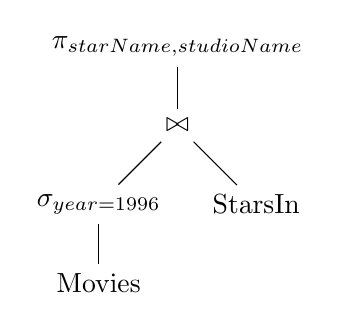
\begin{tikzpicture}
        \node (n1){$\pi_{starName, studioName}$};
        \node[below of=n1] (n2){$\bowtie$};
        \node[below of=n2, xshift = -1cm] (n3){$\sigma_{year=1996}$};
        \node[below of=n2, xshift = 1cm] (n4){StarsIn};
        \node[below of=n3] (n5){Movies};
        \draw[-] (n1) -- (n2);
        \draw[-] (n2) -- (n3);
        \draw[-] (n2) -- (n4);
        \draw[-] (n3) -- (n5);
    \end{tikzpicture}
    \caption{$\sigma$算子下推例子}\label{fig:6-select}
\end{figure}
\begin{figure}[H]
    \centering
    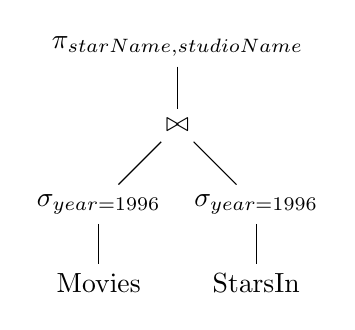
\begin{tikzpicture}
        \node (n1){$\pi_{starName, studioName}$};
        \node[below of=n1] (n2){$\bowtie$};
        \node[below of=n2, xshift = -1cm] (n3){$\sigma_{year=1996}$};
        \node[below of=n2, xshift = 1cm] (n4){$\sigma_{year=1996}$};
        \node[below of=n3] (n5){Movies};
        \node[below of=n4] (n6){StarsIn};
        \draw[-] (n1) -- (n2);
        \draw[-] (n2) -- (n3);
        \draw[-] (n2) -- (n4);
        \draw[-] (n3) -- (n5);
        \draw[-] (n4) -- (n6);
        \end{tikzpicture}
    \caption{$\sigma$算子下推例子2}\label{fig:6-select2}
\end{figure}

在处理$\sigma$下推时，为保证$\sigma$尽可能作用在更多的关系上，优化关系表达式时应该先将$\sigma$上推，然后再下推。

\subsection{投影相关法则}

与下推选择的优化类似，可以下推投影，一般情况下投影也可以减少关系的尺寸。与$\sigma$不同，$\pi$穿透其它算子一般需要引入新的$\pi$，实现中一般会在AST上标注输出属性，根据这个属性可以计算尽可能的做投影。

SQL语句中将属性的表达式也看成投影$\pi_{E \rightarrow x}$，这称为\emph{扩展投影}。扩展投影计算出结果$x$后，将$E$中的属性去掉。例如，扩展投影$\pi_{x+y \rightarrow z}$或者$\pi_{x \rightarrow y}$，实际的SQL语句可能对应于\texttt{SELECT a1+a2 AS b FROM ...}。扩展投影对属性做变换，虽然去掉了$E$中的属性，但并不能保证结果会变小。相对的，将原先的投影定义为\emph{简单投影}，即不涉及属性改名或者没有属性计算的投影$\pi_{E \rightarrow x}$。

对投影做优化的基本思路是：1)~将结果不需要的属性做简单下推投影；2)~扩展投影$\pi_{E \rightarrow x}$尽可能下推；3)~简单投影如果包含在属性$E$中，不能穿透扩展投影。

\begin{itemize}
    \item $\pi_L(R \bowtie S) = \pi_L(\pi_M(R) \bowtie \pi_N(S))$，$M$和$N$是$L$中分别关于$R$和$S$的属性
    \item $\pi_L(R \bowtie_C S) = \pi_L(\pi_M(R) \bowtie_C \pi_N(S))$，$M$和$N$是$L$和$C$中分别关于$R$和$S$的属性
    \item $\pi_L(R \times S) = \pi_L(\pi_M(R) \times \pi_N(S))$，$M$和$N$是$L$中分别关于$R$和$S$的属性
\end{itemize}

上述规则中，$M$和$N$下推投影去除了$\bowtie$、$\bowtie_C$和$\times$运算结果中的无用属性，$\pi_M$和$\pi_N$是两个简单投影。

对于bag模型而言，两个关系的并等价于投影的并：
\begin{itemize}
    \item $\pi_L(R \cup_B S) = \pi_L(R) \cup_B \pi_L(S)$
\end{itemize}
但是set模型没有这个特性。

最后，简单投影可以穿透选择做下推：
\begin{itemize}
    \item $\pi_L(\sigma_C(R)) = \pi_L(\sigma_C(\pi_M(R)))$，$M$是$L$和$C$中依赖的属性
\end{itemize}
这里$M$是简单投影，它表示$L$和$C$中依赖的属性。这个规则没什么用，因为选择会使用iterator管道将投影连接起来处理。

\begin{example}
    以\examplename\ref{exp:6-view}为例，
\begin{lstlisting}[style=verbose]
    CREATE VIEW ParamountMovies AS
        SELECT title, year
        FROM Movies
        WHERE studioName = 'Paramount';
\end{lstlisting}

    这个视表示如下的关系表达式：
    $$\pi_{title, year}(\sigma_{studioName = 'Paramount'}(Movies))$$

    而查询
\begin{lstlisting}[style=verbose]
    SELECT title
    FROM ParamountMovies
    WHERE year = 1979;
\end{lstlisting}

    表示的关系表达式为：
    $$\pi_{title}(\sigma_{year = 1979}(ParamountMovies))$$

\end{example}

\begin{figure}[H]
    \centering
    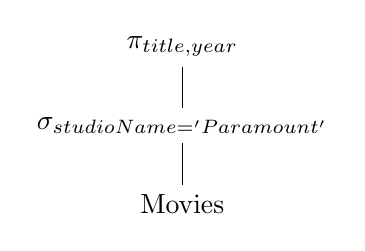
\begin{tikzpicture}
        \node (n1){$\pi_{title, year}$};
        \node[below of=n1] (n2){$\sigma_{studioName = \text{'Paramount'}}$};
        \node[below of=n2] (n3){Movies};
        \draw[-] (n1) -- (n2);
        \draw[-] (n2) -- (n3);
    \end{tikzpicture}
    \caption{视的AST语法树}\label{fig:6-view-tree}
\end{figure}

\begin{figure}[H]
    \centering
    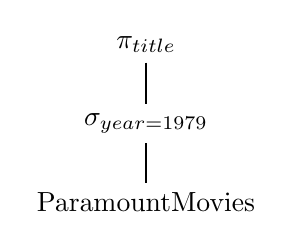
\begin{tikzpicture}
        \node (n1){$\pi_{title}$};
        \node[below of=n1] (n2){$\sigma_{year = 1979}$};
        \node[below of=n2] (n3){ParamountMovies};
        \draw[-] (n1) -- (n2);
        \draw[-] (n2) -- (n3);
    \end{tikzpicture}
    \caption{包含视的AST语法树}\label{fig:6-view-tree2}
\end{figure}

\begin{figure}[H]
    \centering
    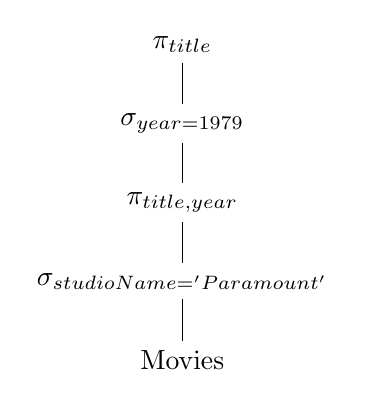
\begin{tikzpicture}
        \node (n1){$\pi_{title}$};
        \node[below of=n1] (n2){$\sigma_{year = 1979}$};
        \node[below of=n2] (n3){$\pi_{title, year}$};
        \node[below of=n3] (n4){$\sigma_{studioName = \text{'Paramount'}}$};
        \node[below of=n4] (n5){Movies};
        \draw[-] (n1) -- (n2);
        \draw[-] (n2) -- (n3);
        \draw[-] (n3) -- (n4);
        \draw[-] (n4) -- (n5);
    \end{tikzpicture}
    \caption{视在语法树上展开}\label{fig:6-view-tree3}
\end{figure}

\begin{figure}[H]
    \centering
    \begin{tikzpicture}
        \node (n1){$\pi_{title}$};
        \node[below of=n1] (n2){$\sigma_{\substack{studioName = \text{'Paramount'} \text{ AND } \\year = 1979}}$};
        \node[below of=n2] (n3){Movies};
        \draw[-] (n1) -- (n2);
        \draw[-] (n2) -- (n3);
    \end{tikzpicture}
    \caption{化简后得到的AST语法树}\label{fig:6-view-tree4}
\end{figure}

\subsection{连接与乘积法则}

根据定义，连接和乘积之间有如下规则：
\begin{itemize}
    \item $R \bowtie_C S = \sigma_C(R \times S)$
    \item $R \bowtie S = \pi_L(\sigma_C(R \times S))$，$C$表示$R$和$S$关系上做连接的同名属性值做相等选择，$L$将两个同名属性去掉一个
\end{itemize}
这里两个规则一般从右向左转化，因为连接比乘积之后的选择要快得多。

如果一个关系自己连接自己：
\begin{itemize}
    \item $R \bowtie R = R$
\end{itemize}

\subsection{副本消除法则}

SQL语言中，一般使用\texttt{DISTICT}关键字表示去重。在在中间计算结果的表上做下推副本消除$\delta$操作可以减小中间表的尺寸，可以加快查询的执行。并且在某些情况下，可以从逻辑上判断直接去掉$\delta$操作：
\begin{itemize}
    \item 聚集存储的关系上声明了主键
    \item set模型上除$\pi$的所有单目操作的计算结果
    \item 当两个关系都是set模型，除$\cup_B$的双目算子计算结果
\end{itemize}

实现上，需要在AST每个节点上设置一个set属性，标记该计算结果是否是set。下推$\delta$可以穿透大多数其它运算：
\begin{itemize}
    \item $\delta(R \times S) = \delta(R) \times \delta(S)$
    \item $\delta(R \bowtie S) = \delta(R) \bowtie \delta(S)$
    \item $\delta(R \bowtie_C S) = \delta(R) \bowtie_C \delta(S)$
    \item $\delta(\sigma_C(R)) = \sigma_C(\delta(R))$
\end{itemize}

对于$\cap$运算，$\delta$可以作用在任意一侧：
\begin{itemize}
    \item $\delta(R \cap S) = \delta(R) \cap S = R \cap \delta(S) = \delta(R) \cap \delta(S)$
\end{itemize}
教材上，交$\cap$是bag模型，其实对set模型也是有效的。这个规则比较有用，与下推$\sigma$类似，它可以先穿越$\cap$上推$\delta$，然后再下推$\delta$。

$\delta$不能穿透$\cup_B$、$-_B$和$\pi$。

\subsection{分组聚合法则}

一般数据库DMBS中，都需要实现\texttt{MIN}、\texttt{MAX}、\texttt{AVG}、\texttt{COUNT}、\texttt{SUM}等几个聚合算法。聚合算法不是普通的函数，它们往往与分组\texttt{GROUP BY}关联，即\texttt{SELECT}的属性列表如果包含了这些聚合函数，则内部实现一般需要分组，而不能看成是扩展投影extending projection。

在实现上，这些聚合函数依赖于分组，即使查询语句中没有显式给出分组\texttt{GROUP BY}，内部也需要根据这些聚合函数的参数做分组。

此外，需要注意的是，聚合计算的结果必然是去重，所以对聚合结果做去重没有意义：
\begin{itemize}
    \item $\delta(\gamma_L(R)) = \gamma_L(R)$，$L$必须包含聚合函数。
\end{itemize}

但是单纯的分组没有上述结论，分组属性$L$中必须包含聚合函数。与上面的结论相对，如果聚合函数是\texttt{MIN}或\texttt{MAX}，去重$\delta$可以穿透分组$\gamma$：
\begin{itemize}
    \item $\gamma_L(R) = \gamma_L(\delta(R))$
\end{itemize}

最后，在\texttt{SELECT}关键字后出现的聚合函数，暗示着类似于投影的语义：
\begin{itemize}
    \item $\gamma_L(R) = \gamma_L(\pi_M(R))$，先对$R$做投影，然后再做分组
\end{itemize}

\begin{example}
    假设两个关系定义如下：
\begin{lstlisting}[style=verbose]
    MovieStar(name, addr, gender, birthdate)
    StarsIn(movieTitle, movieYear, starName)
\end{lstlisting}
    在这两个关系上做如下查询：
\begin{lstlisting}[style=verbose]
    SELECT movieYear, MAX(birthdate)
    FROM MovieStar, StarsIn
    WHERE name = starName
    GROUP BY movieYear;
\end{lstlisting}
    这个查询在\texttt{MovieStar, StarsIn}关系上查找\texttt{name = starName}的元组。虽然在\texttt{GROUP BY}的列表中只有\texttt{movieYear}，但是聚合函数\texttt{MAX}暗示了需要按照\texttt{birthdate}分组。

    这个查询的AST对应于\figurename\ref{fig:6-example-agv}，然后$\sigma(\times(...))$合并成自然连接。\texttt{MAX}函数可以在内部生成一个去重，$\gamma$在内部生成一个投影，得到如\figurename\ref{fig:6-example-agv2}。将$\pi$和$\delta$下推，得到\figurename\ref{fig:6-example-agv3}。

    在\figurename\ref{fig:6-example-agv2}，先在内部生成一个$\pi$，然后再生成一个$\delta$，因为$\delta$无法穿透$\pi$。
\end{example}

\begin{figure}[H]
    \centering
    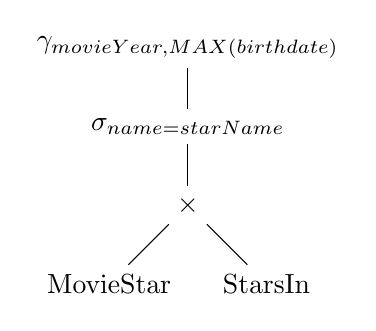
\begin{tikzpicture}
        \node (n1){$\gamma_{movieYear, \text{ MAX}(birthdate)}$};
        \node[below of=n1] (n2){$\sigma_{name=starName}$};
        \node[below of=n2] (n3){$\times$};
        \node[below of=n3, xshift=-1cm] (n4){MovieStar};
        \node[below of=n3, xshift=1cm] (n5){StarsIn};
        \draw[-] (n1) -- (n2);
        \draw[-] (n2) -- (n3);
        \draw[-] (n3) -- (n4);
        \draw[-] (n3) -- (n5);
    \end{tikzpicture}
    \caption{分组聚合示例}\label{fig:6-example-agv}
\end{figure}

\begin{figure}[H]
    \centering
    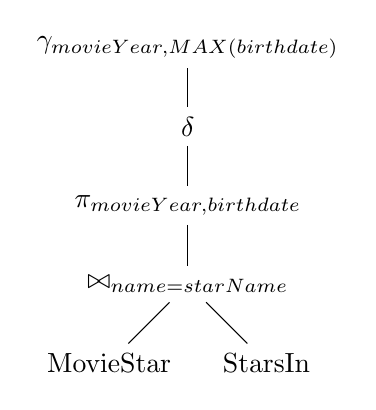
\begin{tikzpicture}
        \node (n0){$\gamma_{movieYear, \text{ MAX}(birthdate)}$};
        \node[below of=n0] (n1){$\delta$};
        \node[below of=n1] (n2){$\pi_{movieYear, birthdate}$};
        \node[below of=n2] (n3){$\bowtie_{name=starName}$};
        \node[below of=n3, xshift=-1cm] (n4){MovieStar};
        \node[below of=n3, xshift=1cm] (n5){StarsIn};
        \draw[-] (n0) -- (n1);
        \draw[-] (n1) -- (n2);
        \draw[-] (n2) -- (n3);
        \draw[-] (n3) -- (n4);
        \draw[-] (n3) -- (n5);
    \end{tikzpicture}
    \caption{分组聚合示例2}\label{fig:6-example-agv2}
\end{figure}

\begin{figure}[H]
    \centering
    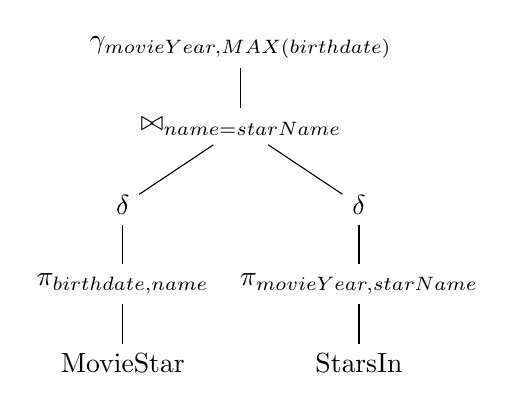
\begin{tikzpicture}
        \node (n1){$\gamma_{movieYear, \text{ MAX}(birthdate)}$};
        \node[below of=n1] (n3){$\bowtie_{name=starName}$};
        \node[below of=n3, xshift=-1.5cm] (n4){$\delta$};
        \node[below of=n3, xshift=1.5cm] (n5){$\delta$};
        \node[below of=n4] (n6){$\pi_{birthdate,name}$};
        \node[below of=n5] (n7){$\pi_{movieYear,starName}$};
        \node[below of=n6] (n8){MovieStar};
        \node[below of=n7] (n9){StarsIn};
        \draw[-] (n1) -- (n3);
        \draw[-] (n3) -- (n4);
        \draw[-] (n3) -- (n5);
        \draw[-] (n4) -- (n6);
        \draw[-] (n5) -- (n7);
        \draw[-] (n6) -- (n8);
        \draw[-] (n7) -- (n9);
    \end{tikzpicture}
    \caption{分组聚合示例3}\label{fig:6-example-agv3}
\end{figure}

\section{算子表达式生成}

SQL语言按照生成式被翻译成CST语法树，在经过类型检查等预处理后，下一步需要将CST变换成抽象语法树AST，AST对应于关系算子表达式。c语言的CST与AST差异不大，但SQL语言中二者有很大差异。在编译原理中，CST转换为AST属于语义分析的范畴，通常采用语法制导翻译。

\subsection{SQL语言}

这里先回顾SQL语言，更详细的内容参见文献\cite{Ullman1998A}第6章。

\subsubsection*{\texttt{SELECT-FROM-WHERE}}

一条简单的\texttt{SELECT-FROM-WHERE}查询语句如下：

\begin{lstlisting}[style=verbose]
    SELECT *
    FROM Movies
    WHERE studioName = 'Disney' AND year = 1990;
\end{lstlisting}

在这条语句中，各个部分的含义是：
\begin{itemize}
    \item \texttt{FROM}指出查询算子作用的关系
    \item \texttt{WHERE}指出查询的条件
    \item \texttt{SELECT}指定输出的字段，对应于投影算子
\end{itemize}

这三个部分与\ref{sec:6-sql}的SQL语法子集中\texttt{<SelectList>}、\texttt{<FromList>}、\texttt{<Con\-dition>}非终止符是对应的。

在SQL-99中，\texttt{SELECT}语句可以利用\texttt{AS}变换输出的属性名称：
\begin{lstlisting}[style=verbose]
    SELECT title, length*0.016667 AS length
    FROM Movies
    WHERE studioName = 'Disney' AND year = 1990;
\end{lstlisting}

\texttt{WHERE}后部的条件是最复杂的部分，SQL-99支持逻辑、算术运算、模式匹配等。

\subsubsection*{\texttt{GROUP BY, ORDER BY}}

使用排序和分组的语句示例如下：
\begin{lstlisting}[style=verbose]
    SELECT *
    FROM Movies
    WHERE studioName = 'Disney' AND year = 1990
    ORDER BY length, title;

    SELECT *
    FROM Movies
    WHERE year = 1990
    GROUP BY sudioName;
\end{lstlisting}

\texttt{GROUP BY, ORDER BY}后面指明分组和排序的属性列表。聚合操作支持\texttt{MIN, MAX, AVG, COUNT, SUM}，这些聚合函数出现在\texttt{SELECT}后的列表中。

\subsubsection*{$\times, \bowtie$}

SQL使用\texttt{FROM}中给出需要处理的多个关系名表示积$\times$。SQL专门设计自然连接\texttt{NATURAL JOIN}和外连接\texttt{OUTER JOIN}关键字，但很少使用，一般表示为乘积，然后由SQL编译器优化为连接或者$\theta$连接。
\begin{lstlisting}[style=verbose]
    SELECT name
    FROM Movies, MovieExec
    WHERE title = 'Star Weirs' AND producerC# = cert#;
\end{lstlisting}

上面的语句中由于使用条件\texttt{producerC\# = cert\#}，表示两个关系的自然连接。所以，要区分出积和连接，是SQL解析器的任务。并且，从SQL语言来看，并没有强制规定算子一定是双目的，可以是多目的。

\subsubsection*{$-, \cap, \cup$}

交并差在SQL中使用关键字\texttt{INTERSECT, UNIION, EXCEPT}表示，如下面的例子：
\begin{lstlisting}[style=verbose]
    (SELECT name, address
     FROM MovieStar
     WHERE gender = 'F'))
    INTERSECT
    (SELECT name, address
     FROM MovieExec
     WHERE netWorth > 10000000);
\end{lstlisting}

\subsubsection*{嵌套子查询}

SQL语法是生成式表述，它支持\texttt{SELECT-FROM-WHERE}语法结构嵌套使用，具体来说嵌套子查询只出现在两个位置：\texttt{FROM}和\texttt{WHERE}。

\begin{itemize}
    \item 子查询的结果可能是一个标量，这个标量可以参与外层查询语句中\texttt{WHERE}中的逻辑表达式计算。
    \item 子查询的结果如果是一个关系，这个关系可以用在\texttt{FROM}和\texttt{WHERE}中。
\end{itemize}

如果查询条件作用在键上，并且\texttt{SELECT}指定只选择一个属性，由于只能选中一行的一个属性，输出结果一定是标量。

\begin{example}
    有两个关系，
\begin{lstlisting}[style=verbose]
Movies(title, year, length, genre, studioName, producerC#)
MovieExec(name, address, cert#, netWorth)
\end{lstlisting}

\texttt{MovieExec}关系的主键是\texttt{cert\#}，然后在这两张表上查询Star Wars电影的制片商
\begin{lstlisting}[style=verbose]
    SELECT name
    FROM Movies, MovieExec
    WHERE title = 'Star Wars' AND producerC# = cert#;
\end{lstlisting}

换一个角度考虑这个问题，由于\texttt{producerC\#}是\texttt{MovieExec}的外键，可以在\texttt{WHERE}条件中指定相等：
\begin{lstlisting}[style=verbose]
    SELECT name
    FROM MovieExec
    WHERE cert# =
        (SELECT producerC#
         FROM Movies
         WHERE title = 'Star Wars');
\end{lstlisting}

后者的的执行效果要好很多，因为可以使用\texttt{Movies}和\texttt{MovieExec}的索引直接输出，而前者如果优化没做好，会使用乘积来处理。
\end{example}

在\ref{sec:6-sql}的语法定义中，\texttt{LIKE}也是作用在单个属性上，它如果嵌套子查询也要求是一个标量。\texttt{IN}后可以嵌套一个子查询，子查询的输出为一个关系。

\begin{example}
    有三张表，
\begin{lstlisting}[style=verbose]
Movies(title, year, length, genre, studioName, producerC#)
StarsIn(movieTitle, movieYear, starName)
MovieExec(name, address, cert#, netWorth)
\end{lstlisting}

在这三张表上查询Harrison Ford参演影片的片商：
\begin{lstlisting}[style=verbose]
    SELECT name
    FROM MovieExec
    WHERE cert# IN
        (SELECT producerC#
         FROM Movies
         WHERE (title, year) IN
            (SELECT movieTitle, movieYear
             FROM StarsIn
             WHERE starName = 'Harrison Ford')
        );
\end{lstlisting}

整个查询嵌套了三层，最内层先在\texttt{StarsIn}上查询Harrison Ford参演的影片，然后在\texttt{Movies}上查询影片的生产商，最后在\texttt{MovieExec}上查询片商的名称。这个查询等价于：
\begin{lstlisting}[style=verbose]
    SELECT name
    FROM MovieExec, Movies, Starsln
    WHERE cert# = producerC# AND
        title = movieTitle AND
        year = movieYear AND
        starName = 'Harrison Ford';
\end{lstlisting}
\end{example}

\subsubsection*{名字解析}

SQL中的名字包括：属性名、表名或者视名。SQL名字解析原则如下：
\begin{itemize}
    \item 在解析SQL语句之前，已创建的表和视，及其属性可见；
    \item \texttt{SELECT-FROM-WHERE}构成一个名字scope；\texttt{FROM}后用\texttt{AS}声明的表实例在这个scope内可见；
    \item 在嵌套子查询中，外层scope的名字可见；
\end{itemize}

\subsection{简单算子表达式构造} \label{sec:6-convert-relation-exp}

\texttt{SELECT-FROM-WHERE}的SQL语法结构包含了投影$\pi$，选择$\sigma$以及乘积$\times$，CST语法树可以利用语法制导翻译出一个$\pi_D(\sigma_C(R \times S \times ...))$或$\gamma_D(\sigma_C(R \times S \times ...))$表达式，其中属性列表$D$由\texttt{SELECT}节点属性给出，条件$C$由\texttt{WHERE}节点属性给出。

这里先讨论最简单的情况：假设\texttt{FROM}和\texttt{WHERE}中没有子查询。条件$C$和$D$的构造是容易的：
\begin{itemize}
    \item 如果只有一个关系则去掉$\times$
    \item 条件$C$即为\texttt{WHERE}中的逻辑表达式
    \item 投影$D$为\texttt{SELECT}中的扩展投影
\end{itemize}

\begin{figure}[H]
    \centering
    \begin{tikzpicture}[node distance = 1cm]
        \node                                   (pi)    {$\pi_D$};
        \node [below of= pi]                    (sigma) {$\sigma_C$};
        \node [below of= sigma]                 (times) {$\times$};
        \node [below of= times, xshift = -1cm]  (R)     {$R$};
        \node [right of= R]                     (S)     {$S$};
        \node [below of= times, xshift = 1cm]   (dot)   {$...$};
        \path (pi)      edge    (sigma);
        \path (sigma)   edge    (times);
        \path (times)   edge    (R);
        \path (times)   edge    (S);
        \path (times)   edge    (dot);
    \end{tikzpicture}
    \caption{将select-from-where构造基本关系表达式}\label{fig:6-construct-relation}
\end{figure}

在实现中，$\times$可以拥有1个或多个子节点，在优化时利用$\sigma_D(R \times S) = R \bowtie_{D} S$将去除$\times$。举例而言，\examplename\ref{exp:6-parse-tree2}的查询语句，它的语法树被翻译成表达式如\figurename\ref{fig:6-example}。

\begin{figure}[H]
    \centering
    \begin{tikzpicture}
        \node (n1){$\pi_{movieTitle}$};
        \node[below of=n1] (n2){$\sigma_{\substack{starName=Name \text{ AND } \\ birthdate \text{ LIKE } '\%1960'}}$};
        \node[below of=n2] (n3){$\times$};
        \node [below of= n3, xshift = -1cm]  (R){StarsIn};
        \node [right of= R, xshift = 1cm] (S){MovieStar};
        \draw[-] (n1) -- (n2);
        \draw[-] (n2) -- (n3);
        \draw[-] (n3) -- (R);
        \draw[-] (n3) -- (S);
    \end{tikzpicture}
    \caption{\examplename\ref{exp:6-parse-tree2}查询语句被翻译为关系表达式}\label{fig:6-example}
\end{figure}

\subsection{\texttt{FROM}嵌套子查询}

当\texttt{FROM}中包含子查询，这个子查询生成的中间结果作为$\times$的一个子节点进行处理，类似于view替换。

\begin{example}\label{exp:6-parse-tree3}
    假设有三个关系定义如下：
\begin{lstlisting}[style=verbose]
    Movies(title, year, length, genre, studioName, producerC#)
    StarsIn(movieTitle, movieYear, starName)
    MovieExec(name, address, cert#, netWorth)
\end{lstlisting}

    在这三个关系上做查询
\begin{lstlisting}[style=verbose]
    SELECT name
    FROM MovieExec, (SELECT producerC#
                     FROM Movies, StarsIn
                     WHERE title = movieTitle AND
                           year = movieYear AND
                           starName = 'Harrison Ford'
                    ) Prod
    WHERE cert# = Prod.producerC#;
\end{lstlisting}

    这条查询语句的算子表达式为\figurename\ref{fig:6-example3}。
\end{example}

\begin{figure}[H]
    \centering
    \begin{tikzpicture}
        \node (n1){$\pi_{name}$};
        \node[below of=n1] (n2){$\sigma_{cert\# = Prod.producerC\#}$};
        \node[below of=n2] (n3){$\times$};
        \node[below of= n3, xshift = -1cm]  (n4){MovieExec};
        \node[right of= R, xshift = 1cm] (n5){$\pi_{producerC\#}$};
        \node[below of=n5] (n6){$\sigma_{\substack{title = movieTitle \text{ AND } \\
        year = movieYear \text{ AND } \\
        starName = \text{'Harrison Ford'}}}$};
        \node[below of=n6, xshift = -1cm] (n7){Movies};
        \node[right of=n7, xshift = 1cm] (n8){StarsIn};
        \draw[-] (n1) -- (n2);
        \draw[-] (n2) -- (n3);
        \draw[-] (n3) -- (n4);
        \draw[-] (n3) -- (n5);
        \draw[-] (n5) -- (n6);
        \draw[-] (n6) -- (n7);
        \draw[-] (n6) -- (n8);
    \end{tikzpicture}
    \caption{\examplename\ref{exp:6-parse-tree3}查询语句被翻译为算子表达式}\label{fig:6-example3}
\end{figure}

\subsection{\texttt{WHERE}属性嵌套子查询}

\texttt{WHERE}后部是选择条件，这个选择条件是$\sigma$算子的下标。\texttt{WHERE}的条件表达式可能嵌套一个子查询，这个子查询在AST中被处理成$\sigma$算子的属性，教材上将它处理成一个\emph{双参}$\sigma$。

\begin{example}\label{exp:6-parse-tree4}
    以\examplename\ref{exp:6-parse-tree}为例，\texttt{WHERE}后的条件\texttt{starName IN}被处理成$\sigma$算子的属性：
    $$\pi_{movieTitle}(\sigma_{starName \in \pi_{name}(\sigma_{birthdate \text{ LIKE } '\%*.1960'}(MovieStar))}(StarsIn))$$
    其中$\pi_{name}(\sigma_{birthdate \text{ LIKE } '\%*.1960'}(MovieStar))$对应于一个中间结果关系，name是这个中间结果的一个属性，表示为\figurename\ref{fig:6-example4}。至于转化为$\times$是一个优化问题，由于$name \in$可以表示为一个等值连接，这个表达式最终被转化为\ref{fig:6-example5}。
    \end{example}

\begin{figure}[H]
    \centering
    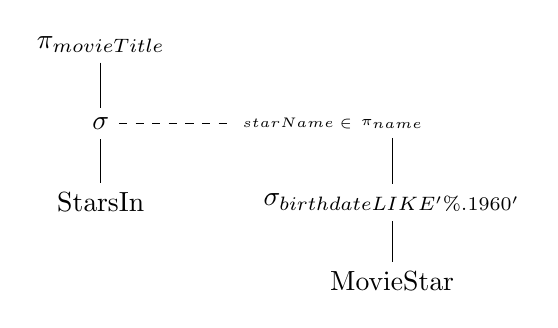
\begin{tikzpicture}
        \node (n1){$\pi_{movieTitle}$};
        \node[below of=n1] (n2){$\sigma$};
        \node[below of=n2] (n3){StarsIn};
        \node[right of=n2, xshift=1.5cm] (n41){\tiny$starName \in$};
        \node[right of=n41, xshift=0.2cm] (n4){\tiny$\pi_{name}$};
        \node[below of=n4] (n5){$\sigma_{birthdate \text{ LIKE '\%.1960'}}$};
        \node[below of=n5] (n6){MovieStar};
        \draw[-] (n1) -- (n2);
        \draw[-] (n2) -- (n3);
        \draw[dashed] (n2) -- (n41);
        \draw[-] (n4) -- (n5);
        \draw[-] (n5) -- (n6);
    \end{tikzpicture}
    \caption{\examplename\ref{exp:6-parse-tree4}查询语句被翻译为算子表达式}\label{fig:6-example4}
\end{figure}

\begin{figure}[H]
    \centering
    \begin{tikzpicture}
        \node (n1){$\pi_{movieTitle}$};
        \node[below of=n1] (n2){$\substack{\bowtie \\ starName=name}$};
        \node[below of=n2, xshift=-1cm] (n3){StarsIn};
        \node[right of=n3, xshift=1cm] (n4){$\pi_{name}$};
        \node[below of=n4] (n5){$\sigma_{birthdate \text{ LIKE '\%.1960'}}$};
        \node[below of=n5] (n6){MovieStar};
        \draw[-] (n1) -- (n2);
        \draw[-] (n2) -- (n3);
        \draw[-] (n2) -- (n4);
        \draw[-] (n4) -- (n5);
        \draw[-] (n5) -- (n6);
    \end{tikzpicture}
    \caption{\examplename\ref{exp:6-parse-tree4}查询语句优化后的算子表达式}\label{fig:6-example5}
\end{figure}

\subsection{相关子查询}

子查询的翻译会碰到一个问题：子查询有可能会引用外部名字，这个名字可能是外部的关系或者属性。如果子查询没有引用外部名字，称子查询是\emph{无关的}，否则称为\emph{相关的}。

与c语言不同，SQL中的名字可以定义在\texttt{SELECT}、\texttt{FROM}或者\texttt{WHERE}中。名字的scope在整个\texttt{SELECT-FROM-WHERE}结构内有效，内层子查询可以引用外部名字。CST在预处理阶段还应该有一个工作：收集该层结构上的所有变量，然后在\texttt{<Query>}节点上标注。

如果内层嵌套子查询引用的外部名字是关系，则意味着这个关系会参与内层嵌套子查询的计算，按照前述的嵌套子查询方式处理。如果引用的是外部关系的属性，这个外部属性一般出现在内层嵌套子查询的\texttt{WHERE}部分，此时问题实质是：内层子查询可能引用外部关系的属性作为条件判断，但是计算总是从内层开始，而外部关系的属性值是未知的。

当内层嵌套子查询的\texttt{WHERE}条件判断出现外部关系的属性，需要利用$\sigma_{C(R,S)}(R) = R \bowtie_{C} S$将选择转化为一个$\theta$连接。

\begin{example}
    假设有两个关系：
\begin{lstlisting}[style=verbose]
    StarsIn(movieTitle, movieYear, starName)
    MovieStar(name, address, gender, birthdate)
\end{lstlisting}

    在\texttt{StarsIn}和\texttt{MovieStar}关系上做如下查询：
\begin{lstlisting}[style=verbose]
    SELECT DISTINCT m1.movieTitle, m1.movieStar
    FROM StarsIn m1
    WHERE m1.movieYear - 40 <= (
        SELECT AVG(s.birthdate)
        FROM StarsIn m2, MovieStar s
        WHERE m2.starName = s.name AND
            m1.movieTitle = m2.movieTitle AND
            m1.movieYear = m2.movieYear
    );
\end{lstlisting}

    这条SQL命令查询影星的平均年龄在40岁之下的电影。先看内部嵌套子查询，这个子查询从StarsIn和MovieStar两个表的连接做查询，其余条件使用了外部变量m1，计算平均生日，然后再利用平均生日去计算外部查询。
    \begin{gather}
        a=m1.movieTitle \notag \\
        b=m1.movieStar \notag \\
        c=m2.starName \notag \\
        d=s.name \notag \\
        e=m2.movieTitle \notag \\
        f=m1.movieYear \notag \\
        g=m2.movieYear \notag \\
        h=s.birthdate \notag \\
        i=\sigma_{a=e \text{ AND } f=g \text{ AND } c=d }(m2 \times s) \notag \\
        j=\gamma_{AVG(h)}(i) \notag \\
        k=\delta(\pi_{a,b}(\sigma_{f-40 \le j}(m1))) \notag
    \end{gather}
    由于\texttt{m1.movie\-Year = m2.movieYear}，可以将之处理成为一个自然连接，得到\figurename\ref{fig:6-example6}。条件$j(m1,m2,s)$处理成一个$\theta$连接，\figurename\ref{fig:6-example7}。
    \begin{gather}
        k_2=\delta(\pi_{a,b}(\sigma_{f-40 \le h}(m1 \times i))) \notag
    \end{gather}
    然后将选择算子$\sigma_{a=e \text{ AND } f=g}$上移与$\times$结合得到连接算子，得到\figurename\ref{fig:6-example8}。$\pi$算子上移后，得到：
    $$m1 \bowtie (m2 \bowtie s)$$
    由于$m1,m2$是同一个关系，最后得到$m1 \bowtie s$，如\figurename\ref{fig:6-example9}。
\end{example}

\begin{figure}[H]
    \centering
    \begin{tikzpicture}
        \node (n0){$\delta$};
        \node[below of=n0] (n1){$\pi_{m1.movieTitle,m1.movieYear}$};
        \node[below of=n1] (n2){$\sigma$};
        \node[below of=n2] (n3){StarsIn m1};
        \node[right of=n2, xshift=1.5cm] (n4){$m1.movieYear-40 \le$};
        \node[right of=n4, xshift=2.2cm] (n5){$\gamma_{AVG(s.birthdate)}$};
        \node[below of=n5] (n6){$\sigma_{\substack{m1.movieTitle = m2.movieTitle \text{ AND }\\ m1.movieYear = m2.movieYear}}$};
        \node[below of=n6] (n7){$\substack{\bowtie \\m2.starName = s.name}$};
        \node[below of=n7, xshift=-1cm] (n8){StarsIn m2};
        \node[right of=n8, xshift=1cm] (n9){MovieStar s};
        \draw[-] (n0) -- (n1);
        \draw[-] (n1) -- (n2);
        \draw[-] (n2) -- (n3);
        \draw[dashed] (n2) -- (n4);
        \draw[-] (n5) -- (n6);
        \draw[-] (n6) -- (n7);
        \draw[-] (n7) -- (n8);
        \draw[-] (n7) -- (n9);
    \end{tikzpicture}
    \caption{相关嵌套子查询举例}\label{fig:6-example6}
\end{figure}

\begin{figure}[H]
    \centering
    \begin{tikzpicture}
        \node (n0){$\delta$};
        \node[below of=n0] (n1){$\pi_{m1.movieTitle,m1.movieYear}$};
        \node[below of=n1] (n21){$\sigma_{m1.movieYear-40 \le AVG(s.birthdate)}$};
        \node[below of=n21] (n2){$\times$};
        \node[below of=n2] (n3){StarsIn m1};
        \node[right of=n3, xshift=3cm] (n6){$\sigma_{\substack{m1.movieTitle = m2.movieTitle \text{ AND }\\ m1.movieYear = m2.movieYear}}$};
        \node[below of=n6] (n7){$\substack{\bowtie \\m2.starName = s.name}$};
        \node[below of=n7, xshift=-1cm] (n8){StarsIn m2};
        \node[right of=n8, xshift=1cm] (n9){MovieStar s};
        \draw[-] (n0) -- (n1);
        \draw[-] (n1) -- (n21);
        \draw[-] (n21) -- (n2);
        \draw[-] (n2) -- (n3);
        \draw[-] (n2) -- (n6);
        \draw[-] (n6) -- (n7);
        \draw[-] (n7) -- (n8);
        \draw[-] (n7) -- (n9);
    \end{tikzpicture}
    \caption{相关嵌套子查询举例2}\label{fig:6-example7}
\end{figure}

\begin{figure}[H]
    \centering
    \begin{tikzpicture}
        \node (n0){$\delta$};
        \node[below of=n0] (n1){$\pi_{m1.movieTitle,m1.movieYear}$};
        \node[below of=n1] (n21){$\sigma_{m1.movieYear-40 \le abd}$};
        \node[below of=n21] (n2){$\bowtie_{\substack{m1.movieTitle = m2.movieTitle \text{ AND }\\ m1.movieYear = m2.movieYear}}$};
        \node[below of=n2] (n3){StarsIn m1};
        \node[right of=n3, xshift=3cm] (n6){$\gamma_{\substack{m2.movieTitle,\\ m2.movieYear, \\AVG(s.birthdate) \rightarrow abd}}$};
        \node[below of=n6] (n7){$\substack{\bowtie \\m2.starName = s.name}$};
        \node[below of=n7, xshift=-1cm] (n8){StarsIn m2};
        \node[right of=n8, xshift=1cm] (n9){MovieStar s};
        \draw[-] (n0) -- (n1);
        \draw[-] (n1) -- (n21);
        \draw[-] (n21) -- (n2);
        \draw[-] (n2) -- (n3);
        \draw[-] (n2) -- (n6);
        \draw[-] (n6) -- (n7);
        \draw[-] (n7) -- (n8);
        \draw[-] (n7) -- (n9);
    \end{tikzpicture}
    \caption{相关嵌套子查询举例3}\label{fig:6-example8}
\end{figure}

\begin{figure}[H]
    \centering
    \begin{tikzpicture}
        \node (n0){$\delta$};
        \node[below of=n0] (n1){$\pi_{m2.movieTitle,m2.movieYear}$};
        \node[below of=n1] (n2){$\sigma_{m2.movieYear-40 \le abd}$};
        \node[below of=n2] (n3){$\gamma_{\substack{m2.movieTitle,\\ m2.movieYear, \\AVG(s.birthdate) \rightarrow abd}}$};
        \node[below of=n3] (n4){$\substack{\bowtie \\m2.starName = s.name}$};
        \node[below of=n4, xshift=-1cm] (n5){StarsIn m2};
        \node[below of=n4, xshift=1cm] (n6){MovieStar s};
        \draw[-] (n0) -- (n1);
        \draw[-] (n1) -- (n2);
        \draw[-] (n2) -- (n3);
        \draw[-] (n3) -- (n4);
        \draw[-] (n4) -- (n5);
        \draw[-] (n4) -- (n6);
    \end{tikzpicture}
    \caption{相关嵌套子查询举例4}\label{fig:6-example9}
\end{figure}

\section{逻辑优化}

在语义分析完毕后，CST转化为一个AST。这个AST的内部节点为各种算子，叶子节点为存储在磁盘上的关系，每个节点上会标注输出属性列表、是否是set模型。与每个子查询\texttt{SELECT-FROM-WHERE}对应，会在该子查询的根节点标注名字列表，实现中可以考虑引入一个特定的节点$\alpha$表示。

逻辑优化的目标至少有两个：1)~变换算子表达式，得到开销最小的算子表达式；2)~消除相关子查询。后者可以通过检查AST的节点属性判断，当发现一个嵌套子查询引用外部关系的属性，可以判断为相关子查询。——这种情况只能出现在\texttt{WHERE}之后，如果出现在\texttt{SELECT}后，CST类型检查会报错。

除了处理相关子查询correlated subquery，逻辑优化的目标是得到开销最小的算子表达式，这要求准确度量一个段子表达式的开销。以\figurename\ref{fig:6-example9}为例计算开销，从根出发，$\delta$建连索引可以支持tuple管道，$\pi$算子支持tuple管道，主要问题在于$\gamma$和$\bowtie$。参考\tablename\ref{tbl:operator-two-pass}，一个算子表达式的开销主要考虑的是$\gamma, -, \times, \bowtie, \bowtie_C$这些不支持tuple管道或者$M$兜不住的算子。进一步，\figurename\ref{fig:6-example9}中$m2 \bowtie s$的开销是可知的，但问题是它的计算结果大小是未知的，从而$\gamma$的开销是未知的。

教材中，估算这个中间计算结果的开销需要利用$V(R,a)$参数，这个统计值由数据库系统周期性的在空闲时扫描全表建立。

逻辑优化的主要方案由两种：1)~直观的规则变换，从原始的AST出发，利用规则对AST上的算子做变换；2)~采用动态规划法，枚举所有规则对算子表达式做变换，估算变换后的算子表达式开销。后者能够得到全局最优解，前者只能得到一个局部最优解。但是，动态规划法存在两个方面的问题：1)~中间计算结果的估算不准确，$V(R,a)$统计值的维护成本很高。2)~存在$R \cap R=R$这样的冗余公式，使得等价算子表达式无穷多，必须将等价算子表达式的解空间降下来。

\subsection{中间结果开销估计}

上一章中，度量一个操作的算法性能主要有两个指标：磁盘IO数量和内存约束。与通常的算法性能评估一致，磁盘IO数量以幂的阶次$O()$来评估。但需要注意，采用多项式幂来评估算子表达式性能，精度是不够的。这也是本小节的目的，希望更精确地给出算子实现算法的性能。

估计中间关系大小需要满足如下几个要求，其中一致性估计比较难以满足。
\begin{itemize}
    \item 准确
    \item 方便
    \item 一致，操作可以采用不同的实现算法，但是中间关系的结果是不变的
\end{itemize}

\subsubsection*{估计投影大小}

不论是简单投影还是扩展投影，都可以准确地推算出$\pi$结果的大小，只是扩展投影要创建新的属性，有可能会增加结果尺寸。

\subsubsection*{估计选择大小}

$\sigma_C$选择的条件有几种：相等、不等、不同。

$\sigma_=$得到的中间结果可以估计为$T(S)=T(R)/V(R,A)$，即对关系$R$的属性$A$做相等选择，平均选择概率是总的记录数目除以属性$A$的不同个数。

$\sigma_<$得到的中间结果可以估计为$T(S)=T(R)/3$，就是$1/3$左右。

$\sigma_{\neq}$得到的中间结果估计为$T(S)=T(R)(V(R,A)-1)/V(R,A)$，即属性$A$的数目减1的概率。

当$\sigma_C$是由\texttt{AND}连接的多个条件，我们可以将之处理为多个$\sigma$级联。这个级联的顺序无所谓，反正结果都是一样的。

$\sigma_{C_1 \text{ OR } C_2}(R)$，如果$C_1$和$C_2$两个条件互相独立，$R$有$n$个记录，$C_1$选择得到了$m_1$个记录，$C_2$选择得到了$m_2$个记录，结果关系的大小为$n(1-(1-m_1/n)(1-m_2/n))$。

$\sigma_{\text{NOT } C}(R)$的中间结果大小为$T(R)$减去$\sigma_C$的估计值。

更准确的估计需要精确掌握$R$关于属性$A$的概率分布，这并不容易做到。教材上介绍了Zipf分布，简单地说，就是2/8律。

实际的选择估计还需要判断条件是否为false，从而导致中间结果大小为0。

\subsubsection*{估计连接的大小}

这里只考虑自然连接，其余的连接按如下规则处理：
\begin{itemize}
    \item 相等连接等同于自然连接，需要考虑的指数属性名字的不同
    \item $\theta$连接等同于$\times$算子后跟一个$\delta$算子，笛卡尔积产生的记录数等于两个关系的记录数目的乘积
\end{itemize}

计算$R(X,Y) \bowtie S(Y,Z)$的大小，主要问题是$Y$在$R$和$S$中是何种关系，例如：
\begin{itemize}
    \item 如果$R$和$S$中的$Y$不相交，则$T(R\times S)=0$
    \item 如果$Y$是$R$的主键，是$S$的外键，则$T(R\times S)=T(R)$
    \item 如果$R$和$S$中的$Y$都相同，则$T(R\times S)=T(R)T(S)$
\end{itemize}

上述例子中，计算连接时结果存在巨大差异。为应付一般性的场景，做如下假设：
\begin{itemize}
    \item 值集包容，如果$V(R,Y) \le V(S,Y)$，则$R$中每个$Y$值都会出现在$S$中。
    \item 值集保持，如果属性$A$是$R$属性但不是$S$的属性，则$V(R\bowtie S,A)=V(R,A)$。
\end{itemize}
值集包容假设并不一定成立，但是在多数情况下是成立的，并且满足$Y$是$S$的主键$R$的外键的情况。值集保持假设也可能不成立，但是对于$Y$是$S$的主键$R$的外键的情况是满足的。值集保持假设在绝大多数情况下是成立的，仅当\emph{dangling tuple}的情况才会出错，即$R$和$S$在属性$Y$上不相交。基于上述假设，自然连接的估计为$T(R\bowtie S)=T(R)T(S)/max(V(R,Y),V(S,Y))$。

当$Y$是多个属性时，估计为$T(R\bowtie S)=T(R)T(S)/max(V(R,y_1),V(S,y_2))$，其中$y_1$使得$V(R,y_1)$最大，$y_2$使得$V(S,y_2)$最大。

多个自然连接的情况$S=R_1 \bowtie R_2 \bowtie ... \bowtie R_n$，先将$T(R_i)$相乘，然后找到所有出现过两次的属性$A$，将乘积除以$V(R_i,A)$（最小的$V(R_i,A)$除外）。

\subsubsection*{估计其它操作大小}

处理前面介绍的投影$\pi$、选择$\sigma$和连接$\bowtie$三种操作外，其余的操作只能凭经验给出估计。

$R \cup_B S$相对容易，$T(R)+T(S)$。$R \cup_S S$不好估计，它的最大值是$T(R)+T(S)$，最小值是$max(T(R),T(S))$，教材中的估计值是$(T(R)+T(S)+max(T(R),T(S)))/2$。

$R \cap S$的最小值是0，最大值是$min(T(R),T(S))$，估计值为$min(T(R),T(S))/2$。

$R-S$的结果在$T(R)$和$T(R)-T(s)$之间，教材给出估计值为$T(R)-T(S)/2$。

\subsubsection*{统计信息收集}

一个关系$R$上的所有统计信息中，$V(R,a)$的信息最难以维持。教材中的主要方法是由一个定期执行的后台程序扫描整个关系，抽取histogram。可以按照等宽、等高、频率收集histogram信息。

这个方案开销太大，一个更好的方案是采用bloomfilter来维护。对每个属性$a$维护一个pair<bloomfilter, count>，新插入一条记录，同时在每个属性的bloomfilter中判断是否出现，如果没有则在count上加1。进一步，pair<bloomfilter, count>可以用Counting BloomFilter代替。Spectral BloomFilter和Dynamic BloomFilter还可以象histogram一样统计各个区段的信息，这些信息可以进一步扩展教材中的预估方案。

\subsection{直观算法}

直观算法从原始AST出发，直接对树型结构做变换。考虑到：1)~等价算子表达式的结果不变；2)~tuple管道的开销不计算。直观算法的目标是减小$\gamma, -, \times, \bowtie, \bowtie_C$算子之间的中间计算结果，尽可能避免中间结果的物化。

例如\figurename\ref{fig:6-example9}，它首先要减少一个$\bowtie_C$，然后可以将$\gamma$对自然连接做投影$\pi$。而投影在AST上的计算，可以从根开始逐步约束其它内部节点。

一般直观算法会写成各种规则，对AST应用这些规则，例如$\sigma,\pi$的下推规则等。直观算法的步骤是：
\begin{enumerate}
    \item 遍历AST树，消除$\sigma$属性上的相关子查询；
    \item 遍历AST树，尝试利用冗余规则减少$\gamma, -, \times, \bowtie, \bowtie_C$算子；
    \item 尝试将$\bowtie, \times, \bowtie_C$转化为$\sigma$条件中的标量；
    \item 标定需要物化的算子，然后尝试利用$\sigma,\pi,\gamma$去缩减该算子的输入中间计算结果；
    \item 尝试利用交换律、结合律确定多目算子$\bowtie, \times, \cap, \cup$的计算顺序；
\end{enumerate}

\subsection{多目算子计算顺序}

$\cap$、$\cup$、$\times$和$\bowtie$这几个算子既满足交换律又满足结合律，这样的操作可以看成是多目操作，执行顺序不影响最终结果，如\figurename\ref{fig:6-assoc-rule}。

\begin{figure}[H]
    \centering
    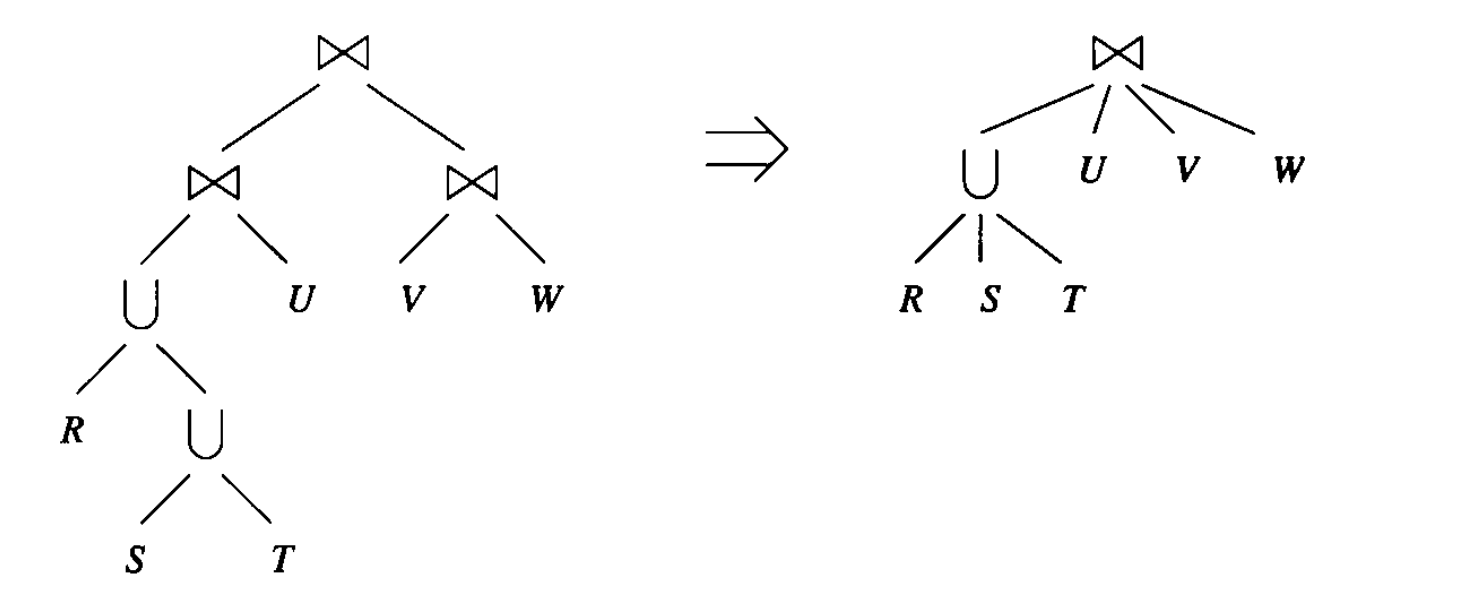
\includegraphics[width=0.8\linewidth]{handout/img/6-assoc-rule.png}
    \caption{可交换可结合的双目操作看成多目操作}\label{fig:6-assoc-rule}
\end{figure}

要确定夺目算子的计算顺序，优化的目标是使总的中间计算结果之和最小，可以使用动态规划来处理这个优化问题。一般是现在都采用贪婪算法，保证下一个的中间结果最小。

在分布式场景中，会假设内存足够大，通过MapReduce、Spark这样的分布式调度方案在各节点上传递数据，由于$\cap, \cup, \times, \bowtie$都支持tuple管道，分布式系统中处理这个问题的手法会不同。

\subsubsection*{左join树}

假设有$m$个关系组合成为一个多目操作，如果不加括号，多目算子的计算顺序等价于一个排列问题$m!$。双目操作的计算顺序落实到join树，有很多种如\figurename\ref{fig:6-join-tree}，其中最左join树对应于一个关系排列。

\begin{figure}[H]
    \centering
    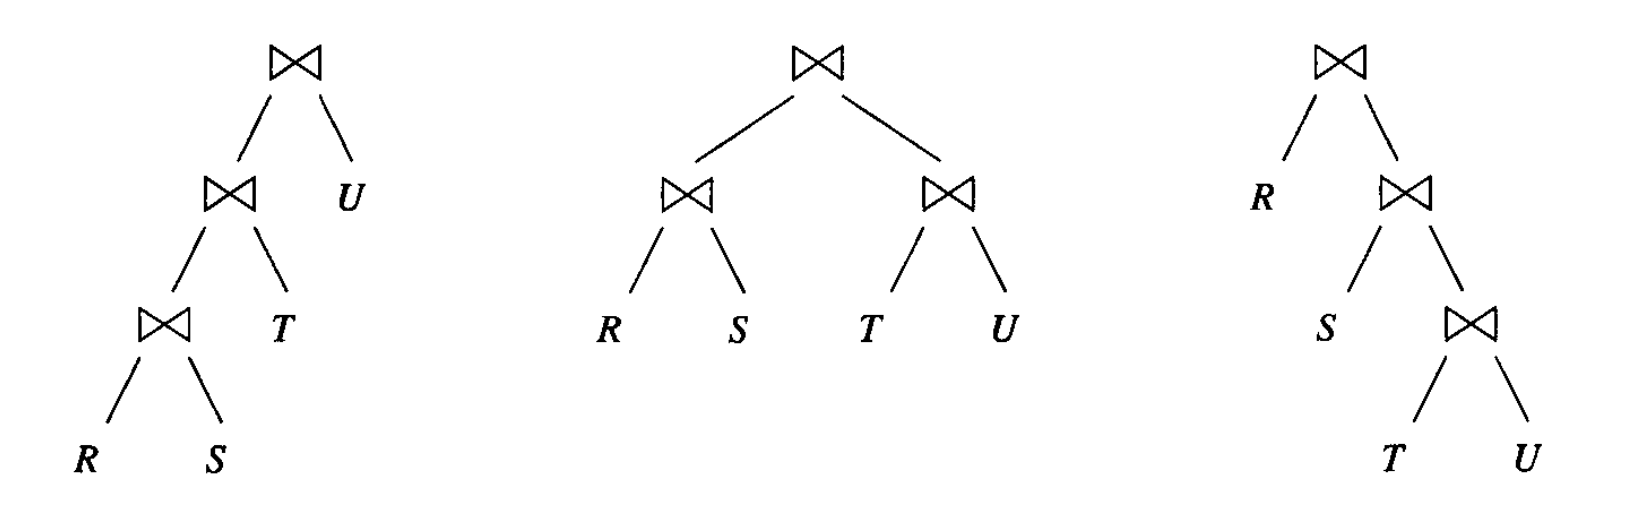
\includegraphics[width=0.8\linewidth]{handout/img/6-join-tree.png}
    \caption{join树}\label{fig:6-join-tree}
\end{figure}

在实现中，上一次$\bowtie$操作的结果不需要物化(merterialization)到磁盘，直接与选定的下一个关系做join操作。

\section{物理优化}

在完成逻辑优化后，得到一棵AST，最后一步是选择AST树上算子的实现算法，连接各算子。按照上一章的说法，算子连接主要有两种：tuple管道和物化。物理优化的主要工作是：1)~选择算子实现算法；2)~处理算子之间的连接。

根据上一章的讨论，主要关注的是$\times, \gamma, \tau, -, \bowtie, \bowtie_C$这些算子的输出，因为它们不支持单轮的tuple管道。具体的算子直接利用上一章的递推多轮算法。

物理优化仍然会在AST上标注，可以采用深度遍历方式处理，如\figurename\ref{fig:6-physical-plan}。

\begin{figure}[H]
    \centering
    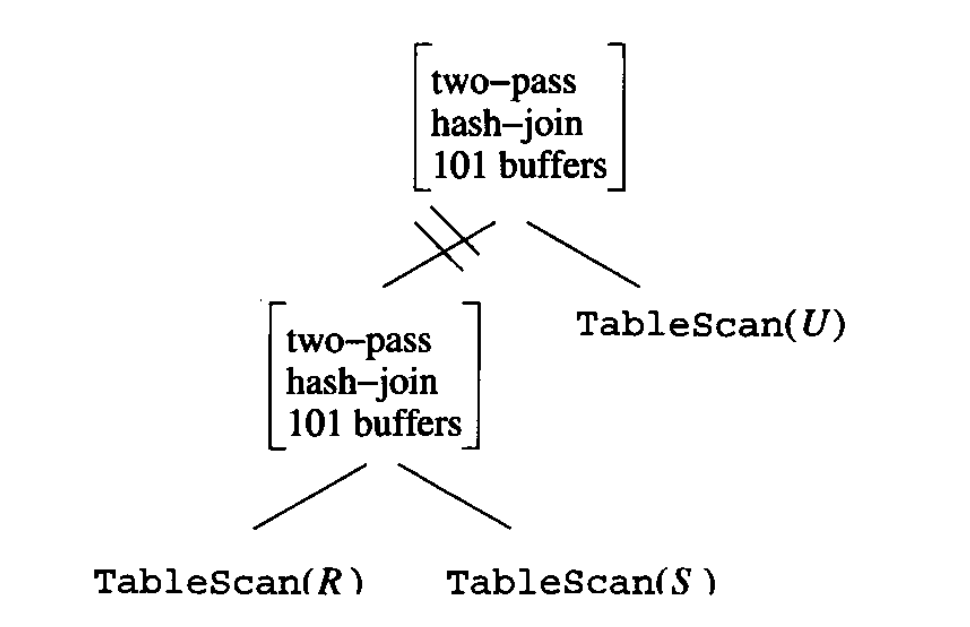
\includegraphics[width=0.6\linewidth]{handout/img/6-physical-plan.png}
    \caption{物理执行计划的树型表示}\label{fig:6-physical-plan}
\end{figure}
